\chapter{\textit{Machine Learning} e Análise de Sentimentos}

\section{Considerações}
\label{sec:considerations}

Ao longo deste capítulo usaremos n para se referir à quantidade de elementos
do conjunto de entrada, cada entrada é i é um vetor $x_i \in \mathbb{R}^m$.
O conjunto de entrada entrada será referida como X
 durante as descrições do algoritmo e assim cada entrada será 
dada tanto como $X_i$ como $x_i$.
Para cada i associaremos duas variáveis $t_i$ e $y_i$ que se referem ao valor
esperado e ao valor obtido através do treinamento, respectivamente.

A notação $\mathds{1}_{i == j}$ é uma função indicadora que vale 1 se i é
igual a j e 0 caso contrário.

\section{Contextualização}
\label{sec:methods}

Os problemas tratados por \textit{Machine Learning} classificam-se de forma
geral em três tipos:

\begin{itemize}
	\item Aprendizado supervisionado: nesse caso tem-se os elementos de entrada e
	para cada um desses elementos, tem-se associado um rótulo $t_i$. Nesse caso o modelo
	deve ser treinado com base nos elementos dados para que se possa prever o rótulo %não consegui pensar numa tradução boa pra label%
	de uma nova entrada;
	\item Aprendizado não-supervisionado: nesse caso tem-se apenas os elementos de entrada. 
	O objetivo deste tipo de problema é tentar modelar uma distribuição ou estrutura comum
	entre os dados para que se possa entendê-los melhor;
	\item Aprendizado semi-supervisionado: nesse último caso alguns elementos possuem um rótulo
	associado. Problemas desse tipo aplicam técnicas gtanto de aprendizado supervisionado como
	de não-supervisionado.
\end{itemize}

Neste trabalho será tratado um problema de aprendizado supervisionado que é o da classificação.

Na classificação temos k classes e cada elemento i da entrada é associado a uma classe $t_i = \{1..k\}$.
O objetivo do problema da classificação é dado entrada $X = (x_1, x_2, \ldots, x_n)$ 
e $t = (t_1, \ldots, t_n)$ treinar um modelo capaz de prever classes para um x qualquer.

Há diversos algoritmos na literatura que se propõem a resolver o problema da classificação.
Bishop (2006)\cite{bishop2006} enuncia diversos dos algoritmos comumente utilizados para a
classificação, cada algoritmo possui seus prós e contras e utiliza diferentes abordagens.

Para este trabalho escolheu-se implementar os algoritmos \textit{Logistic Regression} e
\textit{Support Vector Machines}, que será chamado simplesmente de SVM por facilidade.

Tanto para o \textit{Logistic Regression} quanto SVM será explicado a princípio o problema
será inicialmente abordado a partir da classificação binária e, a partir dela, será descrito
como estender para o problema com mais de duas classes, que será é o caso deste trabalho.

\section{Logistic Regression}
\label{sec:logreg} 

O nosso modelo será construído de forma probabilística, isto é, a partir de um 
discriminante linear $w^Tx + w_0$ atribuiremos uma probabilidade de um elemento x
pertencer à classe $C^1$ e, consequentemente a probabilidade de pertencer à classe
$C^2$ é dada por $1 - P(C^1 | x)$. O termo $w_0$ é chamado de viés, e para efeito
das contas que serão feitas consideraremos vetores w' e x' da forma $x' = (x, 1)$,
$w'= (w, w_0)$ note entretanto que os chamaremos daqui pra frente simplesmente de w e x.

No caso da classificação binária, usaremos que $t_n \in \{0, 1\}$ onde $t_n = 1$ se o
elemento pertence à classe $C^1$ e $t_n = 0$ se pertence à classe $C^2$.

A classificação de um elemento será a classe a qual ele tem maior probabilidade de pertencer.

Para utilizarmos nosso discriminante para atribuir as probabilidades, utiliza-se a função
sigmóide definida por:

\begin{center}
	\begin{equation}
		\sigma(a) = \frac{1}{1 + exp(-a)}
	\end{equation}
\end{center}

A função sigmóide é usada devido à sua propriedade de mapear
todo o conjunto dos números reais dentro do intervalo $[0, 1]$.

Aplicando ao nosso modelo obtêm-se a expressão:

\begin{center}
	\begin{equation}
		P(C^1 | x) = y(x) = \sigma(w^Tx)
	\end{equation}
\end{center}

Importante notar que apesar de utilizarmos o vetor x nas equações, é possível aplicarmos uma
transformação linear $\phi : \mathcal{R}^m \rightarrow \mathcal{R}^d$ à entrada x para obtermos
$\phi(x)$ e usá-lo no lugar de x. O uso de transformação linear no nosso conjunto
de entrada nos permite transformar o domínio para que se obtenha uma separação
melhor entre as classes ou até mesmo fazer a redução da dimensão do domínio.

Com essa equação em mãos, nosso objetivo é minimizar o erro na classificação dos dados. Tomamos
como erro o negativo do logaritmo da verosimilhança de nossa função que é dada por:

\begin{center}
	\begin{equation}
		E(w) = - \sum_{i = 1}^{n} p(t | w) = 
		- \sum_{i = 1}^{n} \{ t_nln(y_n) + (1 - t_n) ln(1 - y_n) \}
	\end{equation}
\end{center}

A fim de minimizar o erro, utiliza-se métodos de otimização linear (note que por mais que se use uma
transformação linear $\phi$ sobre x nosso problema ainda é linear sobre w).

Dois métodos são comumente	usados: método do gradiente e método de Newton-Raphson.
Esses métodos são utilizados tanto para o caso da classificação binária
quanto o caso da classificação com $k > 2$. A diferença entre um problema e outro será abordada
com mais detalhes a seguir.

Uma dúvida natural que surge ao ter que resolver um problema de otimização é o caso de parar o
procedimento em um mínimo local ao invés de um mínimo local da função.	Entretanto, temos que nossa
função $E(w)$ é côncava, isto é, $E(\lambda w + (1 - \lambda ) w') = \lambda E(w) 
	+ (1 - \lambda ) w'$
 $\forall w, w' \in R^m, \lambda \in [0, 1]$, tal propriedade nos garante que existe um único minizador.
 

\subsection{Método do Gradiente}\label{subsec:grad_descent}

Para este método, minimiza-se a função objetivo, no caso $E(w)$ utilizando apenas o gradiente
da função junto de um passo $\alpha$. Com ambos valores em mãos, o valor w é atualizado usando
a equação:

\begin{center}
	\begin{equation}
		w^{ ( novo )} = w^{ (antigo) }  + \alpha \nabla E(w)
	\end{equation}
\end{center}

Com $\nabla E(w)$ sendo o gradiente do vetor de pesos. O gradiente é calculado usando o fato de que
a derivada da função sigmóide com respeito a um vetor a é dada por:

\begin{center}
	\begin{equation}
	\label{eq:sigmoid_derivative}
		\frac{d \sigma}{d a} = \sigma (1 - \sigma )
	\end{equation}
\end{center}

Usando \ref{eq:sigmoid_derivative} tem-se a seguinte equação para o gradiente:

\begin{center}
	\begin{equation}\label{eq:gradient}
		\nabla E(w) = X^T(y - t)
	\end{equation}
\end{center}

Com $y = (y_1, \ldots, y_n)$ e $t = (t_1, \ldots, t_n)$ onde
$y_n = P(C^1 | x_n) = \sigma(w^Tx)$ e $t_n$ tal qual assumido no começo da seção.

O algoritmo de atualização do vetor de pesos descrito a seguir vale tanto para o método
do gradiente quanto para o de Newton-Raphson, portanto para o segundo será focado apenas nas
diferenças entre os dois.


\begin{algorithm}[H]
	\caption{Logistic Regression usando método do gradiente}
	\begin{algorithmic}[1]
		\REQUIRE Matriz $ X \in \mathbb{R}^{n \times m} $, 
		vetor de rótulos $t \in \{0, 1\}^n$
		\ENSURE Vetor de pesos $w \in \mathbb{R}^m$
		\STATE $iteracao \leftarrow 0$
		\STATE $w \leftarrow 0$
		\WHILE{ $|E(w)^{ (iteracao) } - E(w)^{ (iteracao - 1) } | \ge \epsilon$ \AND
		$iteracao < maxIteracoes$ } \label{lst:line:condition}
			\STATE $y \leftarrow (\sigma(w^Tx_1), \sigma(w^Tx_2), \ldots, \sigma(w^Tx_n))^T$
			\STATE $\nabla E(w) \leftarrow X^T(y - t)$
			\STATE $w \leftarrow w - \alpha \nabla E(w)$
			\STATE $E(w)^{ (iteracao) } \leftarrow 
			- \sum_{i = 1}^{n} \{ t_nln(y_n) + (1 - t_n) ln(1 - y_n) \}$
			\STATE $iteracao \leftarrow iteracao + 1$
		\ENDWHILE
	\end{algorithmic}
\end{algorithm}

Importante notar que em~\ref{lst:line:condition} tem-se duas condições de paradas do algoritmo que
são o número de iterações e a diferença da diminuição da função objetivo for menor do que
um dado $\epsilon$. Tais condições são chamadas de condições de convergência e nos garantem
que chegamos a um valor suficientemente próximo do ótimo, uma vez que atingir este valor
pode exigir um número muito alto de iterações o que acarreta em grande custo computacional.
 Na implementação do algoritmo, escolheu-se um valores
padrão para $\epsilon$ e $maxIteracoes$ como $10^{-4}$ e $200$ respectivamente.

A quantidade de iterações necessárias para a convergência é influenciada fortemente pela
escolha de $\alpha$, pois as escolha de um valor pequeno para $\alpha$ acarretaria
em muitas iterações para convergir ao passo que um valor muito grande pode fazer
com que o algoritmo pare num valor distante do ótimo.


\subsection{Método de Newton-Raphson}
\label{subsec:newton-raphson}

Vimos em \ref{subsec:grad_descent} que o método do gradiente apesar de implementação
simples pode levar muito tempo para resolver o problema.

O método de Newton-Raphson acaba convergindo mais rápido do que o método do gradiente,
contudo ao custo de uma maior complexidade devido à necessidade de calcular outros
elementos.

A atualização agora é feita seguindo a equação

\begin{center}
	\begin{equation}\label{eq:newton-raphson}
		w^{ (novo) } = w^{ (antigo) } - H^{-1} \nabla E(w)
	\end{equation}
\end{center}

Onde H é a matriz Hessiano da função erro, que é calculado usando $H = \nabla \nabla E(w)
= X^TRX$ onde R é uma matriz diagonal $n \times n$ onde as entradas da diagonal principal
valem $R_{kk} = y_k(1 - y_k)$. Substituindo os valores de H e usando
\ref{eq:gradient} em \ref{eq:newton-raphson} obtemos


\begin{equation}
\begin{split}
w^{ (novo) } & = w^{ (antigo) } - (X^T R X)^{-1} \nabla E(w) \\
	& = (X^T R X)^{-1}[(X^T R X)w^{ (antigo) } - X^T(y - t)]  
\end{split}
\end{equation}

\subsection{Extensão para o caso de várias classes}

Diversas abordagens podem ser usadas para resolver o problema multiclasse, no
caso será usado diversos discriminantes $y_k$ com $k = \{1, \ldots K\}$ com K
sendo o total de classes. Assim nosso vetor w agora é uma matriz
$W \in \mathbb{R}^{m \times k}$. Outra representação que usaremos para o algoritmo
será $W = (w_1, \ldots, w_k)$ com $w_i \in \mathbb{R}^{1 \times mk}$.

Quanto à codificação do vetor de rótulos, 
segue-se a codificação dada em Bishop (2006)\cite{bishop2006} de $1-K$,
na codificação tem-se que $t_n \in \{0, 1\}^k$ com $t_{nk} = 1$ se o elemento
n pertencer à classe k e 0 nas demais entradas. 

Quanto a função de probabilidade que desejamos estimar, utiliza-se a função
\textit{softmax} que é dada pela equação:

\begin{center}
	\begin{equation}
		P(C^k | x_n) = y_{nk} = \frac{exp(w_k^Tx_n)}{\sum_j exp(w_j^Tx_n)} 
	\end{equation}
\end{center}

Que nos dá verossimilhança e a seguinte função de erro, obtida
tomando o negativo do logaritmo da verossimilhança.

\begin{center}
	\begin{align*}
				P(T | w_1, \ldots, w_k) &= \prod_{i = 1}^{n} \prod_{j = 1}^{k} P(C^j | x_i)^{t_{ij}} = \prod_{i = 1}^{n} \prod_{j = 1}^{k} y_{ij}^{t_{ij}} \\
		E(W) &= - \sum_{i = 1}^{n} \sum_{j = 1}^{k} t_{ij} ln(y_{ij})	
	\end{align*}
\end{center}

Novamente nesse caso pode-se encontrar o valor de W que minimize $E(W)$ usando os
dois métodos discutidos em \ref{subsec:grad_descent} e \ref{subsec:newton-raphson},
porém agora temos que a derivada com respeito a cada $w_k^Tx$ vale:

\begin{center}
	\begin{equation}\label{eq:softmax_derivative}
		\frac{\partial y_k}{\partial (w_j^Tx)} = y_k(\mathds{1}_{k == j} - y_j)
	\end{equation}
\end{center}

Usando essa representação de W como um vetor, podemos calcular o vetor gradiente onde a derivada
com respeito a cada $w_j$ é dada pela equação:

\begin{center}
	\begin{equation}
		\nabla_{w_j} E(W) = X^T(Y_j - T_j)
	\end{equation}
\end{center}

Com $Y_j$ e $T_j$ correspondendo, respectivamente, às j-ésimas colunas de Y e T.

Com o gradiente em mãos já temos o que é necessário para o método do gradiente e a
atualização seria feita da forma $W^{ (novo) } = W^{ (antigo) } - \alpha \nabla E(W)$.

Para aplicarmos o método de Newton-Raphson, seria necessário computarmos o Hessiano que
nesse caso seria uma matriz $m*k \times m*k$ com cada bloco $j, i$ contendo uma matriz
$m \times m$ calculada pela equação:

\begin{center}
	\begin{equation}
		\nabla_{w_i} \nabla_{w_j} E(W) = - \sum_{k = 1}^n y_{ki}( \mathds{1}_{i == j} - y_{kj})
		X_k^TX_k
	\end{equation}
\end{center} 

Onde $X_k$ é a k-ésima linha de X. Com essas equações em mãos nossa atualização de
W seria feita usando a fórmula $W^{ (novo) } = W^{ (antigo) } - H^{-1}\nabla E(W)$.

A classificação de um novo x é feita a partir
do cálculo de $P(C^k | x) = y_k(x), \forall k = \{1, \ldots, k\}$.

A classe de x é dada pelo k que tiver a maior probabilidade sobre os demais.


\section{Support Vector Machine}

Assim como fizemos com o logistic regression, começaremos com a definição
para o caso binário e depois iremos estender para mais de uma classe. Nesse caso
nossas classes serão $t_n \in \{-1, 1\}$ onde $t_n = 1$ se x pertence à classe $C^1$ e
$t_n = -1$ se x pertence à classe $C^2$.

No algoritmo SVM a classificação é feita a partir de um discriminante linear
da forma 

\begin{center}
	\begin{equation}\label{eq:svm-discriminant}
		y(x) = w^Tx + b
	\end{equation}
\end{center}

Tal y é chamado de superfície de decisão e a classificação é baseada no sinal de
y. Se $y(x) > 0$, x é atribuído à classe $C^1$, caso contrário é atribuído à classe
$C^2$.

Porém ao invés de procurarmos um w que separe perfeitamente todas as classes (que
não necessariamente existe), nosso objetivo é maximizar a margem do discriminante
linear, isto é, a menor distância de um ponto à superfície. A distância de um ponto à
superfície é dado pela fórmula

\begin{center}
	\begin{equation}
		\frac{[t_n(w^Tx_n + b)]}{||w||}
	\end{equation}
\end{center}
 
Na descrição inicial do problema vamos tratar o caso com o conjunto X linearmente separável, 
o que indica que é possível obter uma superfície que separe sem erro todas as classes para, em
seguida, tratarmos o caso real que é o do conjunto que não é linearmente separável.
O fato de o conjunto ser linearmente separável nos garante que $t_ny(x_n) >0 \forall n$.


\begin{center}
	\begin{equation}
		\argmax_{x, b} \left\{ \frac{1}{||w||} min_n [t_n(w^Tx_n + b)] \right\}
	\end{equation}
\end{center}


Podemos ajustar w e b de forma a termos que $t_n(w^Tx_n + b) = 1$ para o ponto mais
próximo da margem e $t_n(w^Tx_n + b) \ge 1, \forall n$. Com esse reajuste temos que nosso
problema de encontrar um vetor de pesos de margem maximizada seria de maximizar 
$\frac{1}{||w||}$ que é equivalente ao problema de otimização quadrática:

\begin{center}
	\begin{equation}
		\begin{array}{ll@{}ll}
				\argmin_{w, b} & ||w||^2 &\\
				\textbf{sujeito a}& t_k(w^Tx_k + b), &&k = 1, \ldots ,n 
		\end{array}
	\end{equation}
\end{center}

Agora iremos supor que não necessariamente nossa entrada não é linearmente separável, 
isto é, não existe uma superfície de decisão que separe perfeitamente as duas classes. Assim
iremos permitir que alguns valores estejam classificados incorretamente, para isso
será necessário suavizarmos nossa margem penalizando cada uma das entradas incorretamente
classificadas. Cortes e Vapnik (1995)\cite{cortesVapnik1995} descrevem a penalização
através da introdução de variváveis de folga $\xi_n \ge 0$ para cada elemento de X.
Um elemento corretamente classificado teŕa $\xi_n = 0$, os demais pontos têm
 $\xi_n = |t_n - y(x_n)|$.
 
Com isso nossa restrição de $t_ny(x_n) \ge 1$ é modificada e tem-se 
$t_ny(x_n) \ge 1 - \xi_n \forall n$.

O valor de $\xi_n$ assim nos indica três possíveis casos:

\begin{itemize}
	\item Se $\xi_n = 0$, $x_n$ está corretamente classificado e se encontra
	ou na margem ou do lado correto dela.
	\item Se $0 < \xi_n \le 1$, $x_n$ está corretamente classificado e se encontra
	entre a margem e a superfície.
	\item Se $\xi_n > 1$, $x_n$ não está classificado corretamente.
\end{itemize}

A função objetivo agora precisa conter os valores de $\xi$ e para isso colocamos
uma constante $C > 0$ que define a compensação entre a penalização das variáveis de
folga e a margem. Com isso temos o seguinte problema de otimização quadrática:

\begin{center}
	\begin{equation}
		\begin{array}{ll@{}ll}
			\argmin_{w, b, \xi} & C\sum_{i = 1}^n\xi_i + \frac{1}{2}||w||^2 &\\
			\text{sujeito a}& t_k(w^Tx_k + b) \ge 1 - \xi_k, && k = 1, \ldots, n
		\end{array}
	\end{equation}
\end{center}

Para implementar o SVM basta então resolver o problema de otimização quadrática
acima. Isto é feito seguindo os seguintes passos

\begin{enumerate}
	\item Introduz-se multiplicadores de Lagrange $\alpha_n$ e $\mu_n$ e obtem-se o 
	Lagrangiano com as restrições
		\begin{dgroup}
			\begin{dmath}
				L(w, b, \xi) = \frac{1}{2}||w||^2 + C\sum_{i = 1}^n\xi_i - \sum_{i = 1}^n \alpha_i\{t_i(w^Tx_i + b) - 1 + \xi_i\} - \sum_{i = 1}^n \mu_i \xi_i
			\end{dmath}
			\begin{dmath}
				\alpha_n \ge 0
			\end{dmath}
			\begin{dmath}
				t_ny(x_n) - 1 + \xi_n \ge 0
			\end{dmath}
			\begin{dmath}
				\alpha_n\{t_n(w^Tx_n + b) - 1 + \xi_n\} = 0
			\end{dmath}
			\begin{dmath}
				\mu_n \ge 0
			\end{dmath}
			\begin{dmath}
				\mu_n \xi_n = 0
			\end{dmath}
		\end{dgroup}
	\item Derivamos o lagrangiano com respeito a w, b e $\xi$ e igualamos a 0 para obtermos 
	os valores ótios para essas variáveis e, assim obtemos os seguintes valores:
		\begin{gather}
				\frac{\partial L}{\partial w} = 0 \Rightarrow w = \sum_{i = 1}^n \alpha_i t_i x_i \\
				\frac{\partial L}{\partial b} = 0 \Rightarrow \sum_{i = 1}^n \alpha_i t_i  = 0 \\
				\frac{\partial L}{\partial \xi} = 0 \Rightarrow \alpha_n = C - \mu_n 
		\end{gather} 
	\item Com isso em mãos, resolve-se não o problema primal e sim o dual (utiliza-se aqui o fato 
	de que se as condições mencionadas no item anterior são satisfeitas, tem-se que vale
	a dualidade forte e o valor ótimo de ambas as funções coincide). O dual é dado pelo problema
		\begin{center}
			\begin{equation}
				\begin{aligned}	
				& \underset{\alpha}{\text{min}}
				& & \tilde{L}(\alpha) = \sum_{i = 1}^n \alpha_i - 1/2 \sum_{i = 1}^n \sum_{j = 1}^n \alpha_i\alpha_j t_i t_j k(x_i, x_j) \\
				& \text{sujeito a}
				& & 0 \le \alpha_i \le C, i = 1, \ldots, n \\
				&&& \sum_{i = 1}^n \alpha_i t_i = 0 
				\end{aligned}
			\end{equation}
		\end{center}
	No problema a cima é importante destacar a expressão $k(x_i, x_j)$, essa expressão é um
	\textit{Kernel} que é uma função onde $k(x, x') = \phi(x)^T\phi(x')$ com $\phi$ sendo
	alguma transformação linear. Tal qual no caso da regressão logística, essas
	transformações são usadas para mudar o domínio da entrada x.
	\item Acha-se o valor de b usando a fórmula:
		\begin{center}
			\begin{equation}
				b = \frac{1}{N_{\mathcal{M}}} \sum_{n \in \mathcal{M}} \left( t_n - \sum_{m \in \mathcal{S}} \alpha_m t_m k(x_n, x_m) \right)
			\end{equation}
		\end{center}
	Com $\mathcal{M}$ sendo o conjunto de pontos que satisfazem $0 < \alpha_n < C$ e 
	$\mathcal{S}$ o conjunto de vetores de suporte (pontos que possuem $\alpha_n > 0$ e,
	consequentemente, contribuem para a classificação do modelo).
\end{enumerate}

Uma vez resolvido o problema dual e encontrado valor de b, podemos classificar um novo
x usando o sinal do discriminante $y(x)$ dado por
\begin{center}
	\begin{equation}
		y(x) = \sum_{i = 1}^n \alpha_i t_i k(x, x_i) + b = \sum_{n \in \mathcal{S}} \alpha_n t_n l(x, x_n) + b
	\end{equation}
\end{center}

\subsection{Extensão ao caso de multiclasses}

Diversas abordagens são possíveis para o caso de multiclasses. A escolhida entre elas
foi o método intuitivo chamado \textit{One-versus-all} (OVA). Nesse método é construído
K classificadores, com K sendo o número de classes. Cada classificador $y_k$ define uma
superfície de decisão que separa a classe k das demais (por isso o nome \textit{One-versus-all}).
Um novo x tem sua classe dada pela que o classificador $y_k$ tem maior valor, isto é

\begin{center}
	\begin{equation}
		y(x) = \argmax_{k} y_k(x)
	\end{equation}
\end{center}

Portanto a classificação multiclasses se utiliza de todos os recursos já apresentados no caso
binário o que torna simples a construção do classificador.

Na imagem abaixo é mostrado a ideia por trás do método OVA nele a classe $C^1$ é dada pelos círculos,
$C^2$ pelos triângulos e $C^3$ pelas cruzes.
As figuras em vermelho em cada classificador são os pontos onde $t_n = -1$.

\begin{figure}[ht] 
  \begin{subfigure}[b]{0.5\linewidth}
    \centering
    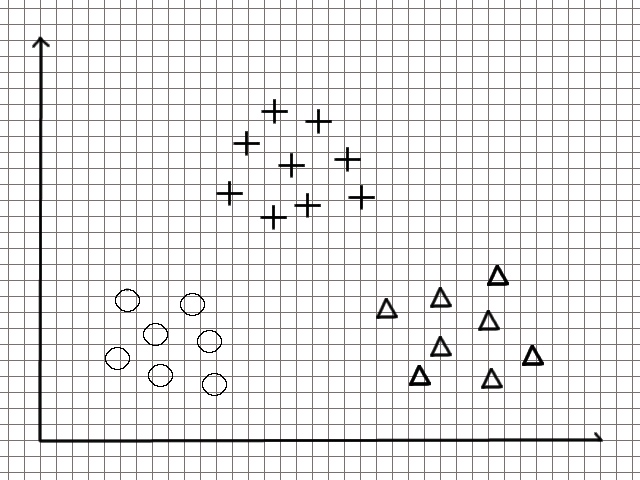
\includegraphics[width=0.75\linewidth]{multiclass_original} 
    \caption{Classes originais} 
    \vspace{4ex}
  \end{subfigure}%% 
  \begin{subfigure}[b]{0.5\linewidth}
    \centering
    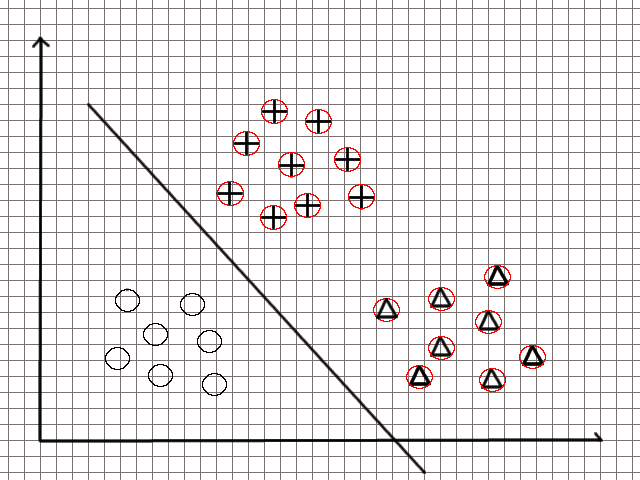
\includegraphics[width=0.75\linewidth]{multiclass_ova1} 
    \caption{Classificador para a classe 1} 
    \vspace{4ex}
  \end{subfigure} 
  \begin{subfigure}[b]{0.5\linewidth}
    \centering
    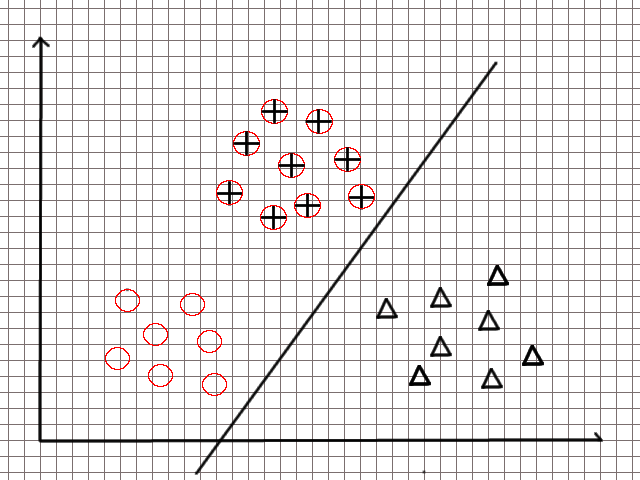
\includegraphics[width=0.75\linewidth]{multiclass_ova2} 
    \caption{Classificador para a classe 2} 
  \end{subfigure}%%
  \begin{subfigure}[b]{0.5\linewidth}
    \centering
    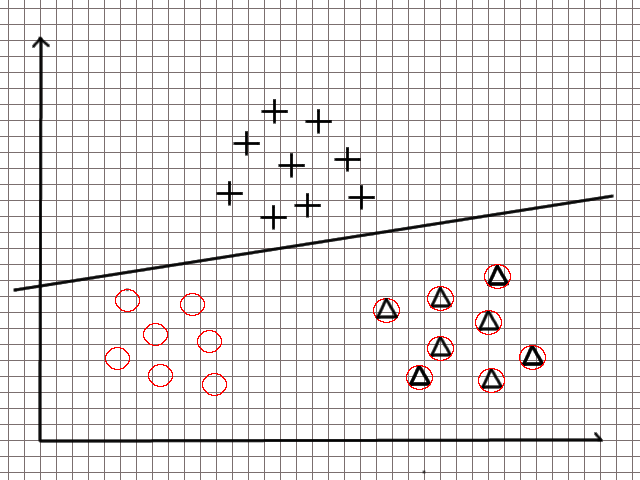
\includegraphics[width=0.75\linewidth]{multiclass_ova3} 
    \caption{Classificaodr para a classe 3} 
  \end{subfigure} 

\end{figure}

\section{Análise de Sentimentos}

O campo de análise de sentimentos, também conhecido como mineração de opinião é uma área da
ciência da computação que analisa as opiniões, sentimentos e atitudes das pessoas em relação
a uma entidade (Bing Liu, 2012)\citep{bingliu2012}. Uma entidade pode ser definida como o sujeito ao qual está
se observando as opiniões, seja ela uma pessoa, instituição ou produto.

A área possui uma diversa gama de aplicações, dentre elas, a área de classificação de sentimentos
que através do uso de informações subjetivas contidas num texto avalia qual a opinião relacionada
ao mesmo.

Classificação de sentimentos teve um crescimento devido à expansão da Web 2.0 que fez com que
as pessoas manifestassem suas opiniões e sentimentos através de blogs, fóruns, redes sociais
e páginas de reviews de produtos que, consequentemente fez com que empresas e pessoas de interesse
tivessem um acesso mais aberto e fácil a essas opiniões. O fácil acesso às opiniões dos usuários
junto com o grande volume delas tornou a análise manual um processo muito custoso, tornando
necessário recorrer a métodos automatizados para a análise e sumarização desses dados que
acabou por fim impulsionando estudos na área (Petković e Ringsquandl, 2013)\citep{petkovic2013}.

Bing Liu, 2012\cite{bingliu2012} divide as formas de classificar sentimentos 
em um documento pode se dividir em quatro formas:
\begin{itemize}
	\item Entidade:  um produto, pessoa sobre o qual o texto se refere, seja direta ou indiretamente.
	Nessa tarefa procura-se analisar se a opinião do texto em torno de uma entidade é positiva ou
	não.
	\item Aspecto: características sobre uma entidade. Por exemplo se temos uma entidade que é um
	produto, aspectos de um produto poderiam ser material ou preço. Nessa forma procura-se avaliar
	a opinião acerca de cada um dos aspectos.
	\item Sentença: esse tipo de análise trabalha com o sentimento associado a cada sentença de
	um documento.
	\item Documento: nesse caso analisa-se o sentimento associado a um documento como um todo, 
	tratando de uma forma mais genérica em relação aos demais.
\end{itemize}

Comum a todas as formas de se analizar as opiniões de um documento é que o uso dos métodos
para obter a opinião. Há duas abordagens para esse problema de classificação: a de aprendizado
de máquina (que iremos utilizar nesse trabalho) que se consiste do uso de algoritmos de 
classificação em conjunto com técnicas de processamento de texto (que será explicado nas próximas
seções) e a abordagem com um dicionário léxico onde a análise é feita baseada na pontuação
entre palavras positivas e negativas contidas no documento (Medhat et al., 2014) \citep{medhat2014}.

No caso desse trabalho, foi escolhido a análise em torno do documento / sentença (devido à estrutura
dos \textit{tweets} tem-se que os documentos são, em sua maioria, compostos por apenas uma 
sentença). 

\subsection{Análise de \textit{Tweets} de política}

Dentre os domínios de aplicação da classificação de sentimentos, escolheu-se como domínio o
escopo político. Nesse caso, temos que as entidades nos documentos são constituídas por
políticos e projetos de lei. E neste trabalho será analisado a análise de \textit{tweets}.

O twitter desde as eleições presidenciais estadunidenses de 2008 mostrou influência
na decisão das eleições evidenciado pela campanha online realizada pela equipe do
candidato Barack Obama (Petković e Ringsquandl, 2013)\citep{petkovic2013}. Desde então, 
a rede social tem sido usada não só para a campanha de políticos, mas também para a avaliação
da opinião em relação às medidas tomadas por eles.

A escolha dos \textit{tweets} foi feita tendo em vista o uso da rede social 
para expressar opiniões sobre diversos assuntos, incluindo política.


\subsection{Obtendo um vetor de \textit{features}}
\label{subsec:featurization}

Para realizar a extração das informações do texto, existe uma etapa de pré-processamento na qual
cada texto é transformado num vetor numérico para então ser processado por algum algoritmo de
classificação. Neste trabalho foi escolhido usar o modelo \textit{bag of words} (BOW). No modelo, 
é construída uma matriz de entrada onde cada linha i representa um documento (texto sobre o qual
quer extrair a opinião) e as colunas representam a frequência de um termo, o conjunto de todos os textos é chamado de \textit{corpus}.

Uma alternativa ao BOW seria o modelo de N-grama, nele os termos não são apenas as palavras, mas
um conjunto de n palavras juntas, o que traz mais informação pelo fato de juntar substantivo e verbo, substantivo e adjetivo, por exemplo, entretanto acaba gerando um vetor de \textit{features}
ainda maior que, consequentemente, faz com que os algoritmos demorem mais para convergir.
A escolha pelo BOW foi tida baseada no compromisso entre desempenho e performance do algoritmo.

Antes de obter um vetor numérico, é feito um pré-processamento no documento removendo artigos, 
adicionando espaços antes e depois de pontuações e transformando em um vetor de tokens. Uma
vez que foi obtido o vetor de \textit{tokens}, é removido todo elemento que seja apenas espaço e pontuação.
Em seguida, monta-se uma nova \textit{string} juntando todas as \textit{tokens} usando espaços
para então montar um vetor de frequência a partir do novo \textit{corpus}.

A frequência pode ser medidas simples como a quantidade de vezes em que um termo j aparece no documento
i ou se o termo j aparece no documento i (nesse caso cada vetor de entrada seria um vetor binário) bem
como pode ser uma medida mais complexa como tf-idf (\textit{term frequency - inverse document frequency}).
A relação entre os métodos de computar a frequência e o desempenho dos algoritmos de classificação serão
exibidas no capítulo seguinte.

O método tf-idf baseia-se na frequência de cada termo ponderada pela frequência inversa no documento,
que é usada para mensurar o quão importante um termo é em um documento (por exemplo a palavra "um" em
um conjunto de textos em português aparece várias vezes, apesar de ter uma baixa importância).
Ele pode ser calculado pelas expressões:

\begin{center}
	\begin{dgroup}
		\begin{dmath}
			TF(t) = \frac{\text{\# de aparições de t no documento}}{\text{total de termos no documento}} 
		\end{dmath}
		\begin{dmath}
			IDF(t) = log \left(  \frac{\text{Total de documentos}}{\text{\# de documentos que contenham t}} \right) 
		\end{dmath}	    
		\begin{dmath}
			TF-IDF(t) = TF(t)*IDF(t)
		\end{dmath} 	    
	\end{dgroup}
\end{center}

O procedimento de obtenção dos vetores de \textit{features} a partir do novo \textit{corpus} pode
ser realizado utilizando as bibliotecas \texttt{scikit-learn} e \texttt{nltk} do Python.

\subsection{Classificação Manual da Opinião}

Com o conjunto de dados obtido em \ref{subsec:featurization}, podemos aplicar os algoritmos 
descritos no começo do capítulo. Entretanto como também mencionado no começo deste capítulo,
problemas de aprendizado supervisionado exigem que o conjunto de dados seja composto não só dos
dados, mas também do valor esperado para cada entrada. No caso da classificação da opinião de
textos, tal opinião deve ser primeiro atribuída manualmente para que, com posse dessas opiniões,
seja possível treinar os algoritmos.

Para facilitar a etapa de classificação manual, foi desenvolvido um sistema online onde cada usuário
informa a quantidade de \textit{tweets} que se deseja classificar e consegue classificá-los de forma
mais simples. Deu-se a essa ferramenta o nome de CLAM (de Classificador Manual).

O desenvolvimento do CLAM foi motivado pela ausência de ferramentas no Brasil que permitem a
colaboração nessa etapa de classificação manual (uma ferramenta comumente usada é o \textit{Amazon
Mechanical Turk}, porém na época do desenvolvimento do CLAM não estava disponível no Brasil)
em conjunto com a falta de ferramentas gratuitas de 
uma forma geral, uma vez que até que a maioria das ferramentas existentes são pagas (vide o 
próprio \textit{Amazon Mechanical Turk}). Por isso priorizou-se construir um código simples
para que fosse fácil a modificiação da base do sistema por colaboradores externos,
que fosse de fácil uso para o usuário final e também de fácil hospedagem do sistema
em alguma plataforma como Heroku e Firebase.

O código é de domínio público e está disponível no link:
 \url{https://github.com/romaolucas/manual-classifier-helper}

O projeto foi desenvolvido usando a linguagem Python em conjunto do \textit{framework} web
Django por já possuir diversas ferramentas integradas não só de gerenciamento do sistema, bem como
modelagem do banco de dados e sistema de migração para que possa modificar os modelos de dados já
existentes sem precisar realizar um acesso direto à base de dados além de possuir um conjunto
de bibliotecas que facilitam o processo de importação de dados em csv e vasta quantidade de 
tutoriais de como desenvolver uma aplicação usando Django.

Para a modelagem de dados construiu-se dois modelos: um para \textit{tweets} e outro para
as opiniões.
Na modelagem, considerou-se que cada usuário irá classificar apenas textos que não 
possuem uma classificação, não só para evitar ter que lidar com opiniões divergentes em um texto,
mas também para garantir um maior número de dados para o treinamento. Uma possível melhoria
do sistema seria a possibilidade de mais usuários avaliarem um mesmo conjunto de textos para
garantir um consenso na hora de associar uma opinião a um texto.

O CLAM possui o seguinte fluxo para a classificação:

\begin{enumerate}
	\item Informa a quantidade de \textit{tweets} que se deseja classificar.
	\begin{figure}[H]
		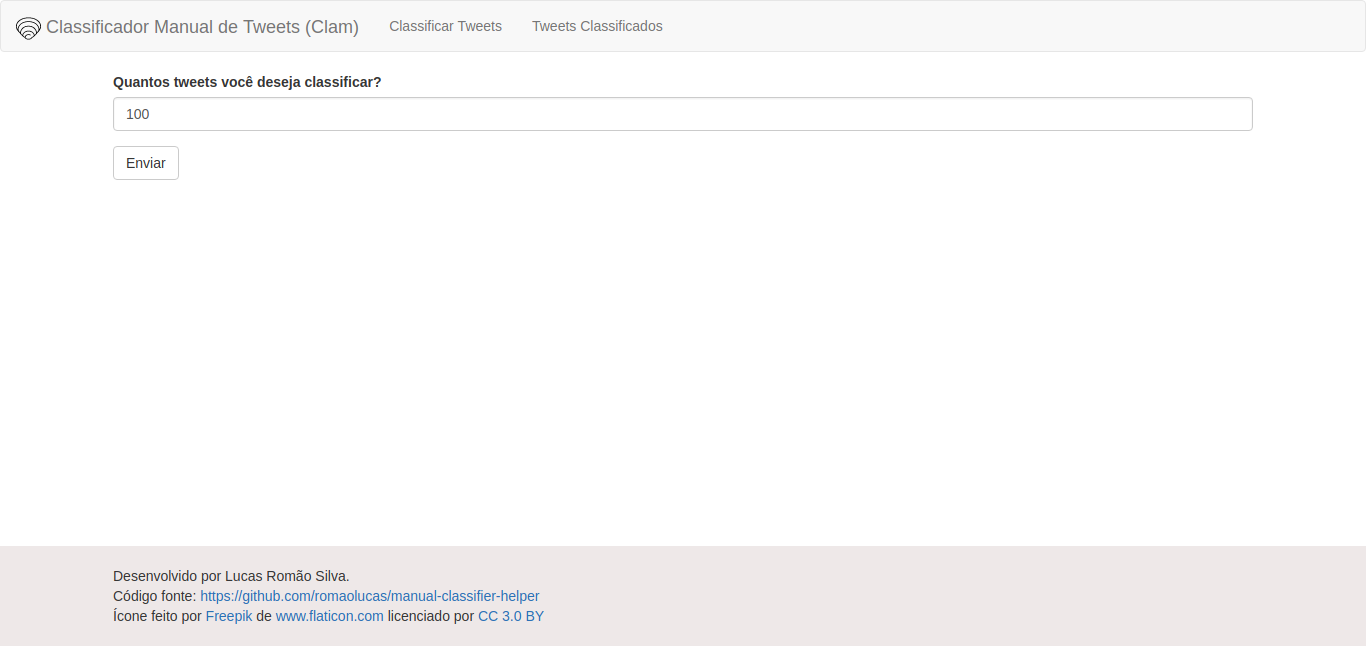
\includegraphics[scale=0.27]{clam_inicio}
	\end{figure}
	\item O usuário é levado a uma página com os n \textit{tweets} para classificar.
	Enquanto o campo da opinião é obrigatório, existe um campo optativo para informar
	se o dado \textit{tweet} é irônico ou não, uma vez que textos com ironia atrapalham
	o treinamento por conter palavras positivas sendo usadas de maneira negativa e vice-versa.
	\begin{figure}[H]
		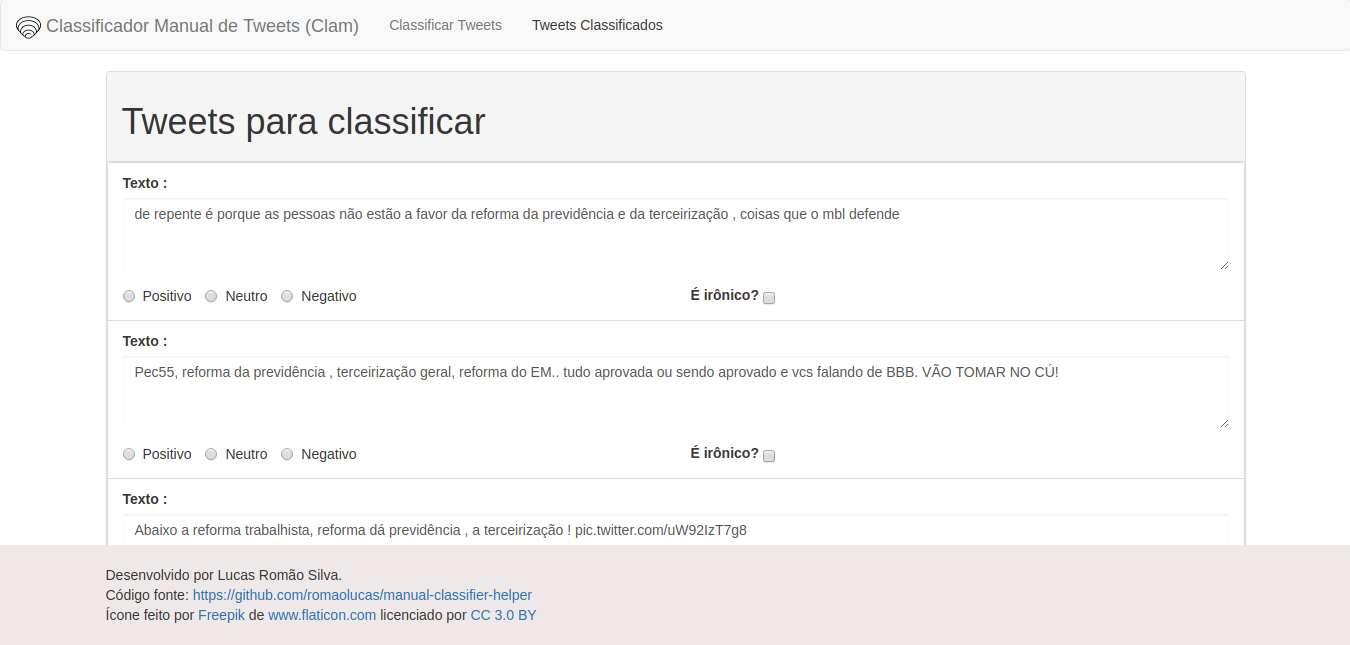
\includegraphics[scale=0.27]{clam_classificar}
	\end{figure}
	\item Uma vez classificados, o usuário é levado a uma página onde é possível ver todos
	os \textit{tweets} já classificados e também gerar um arquivo csv contendo todos aqueles
	que não foram marcados como irônicos.
	\begin{figure}[H]
		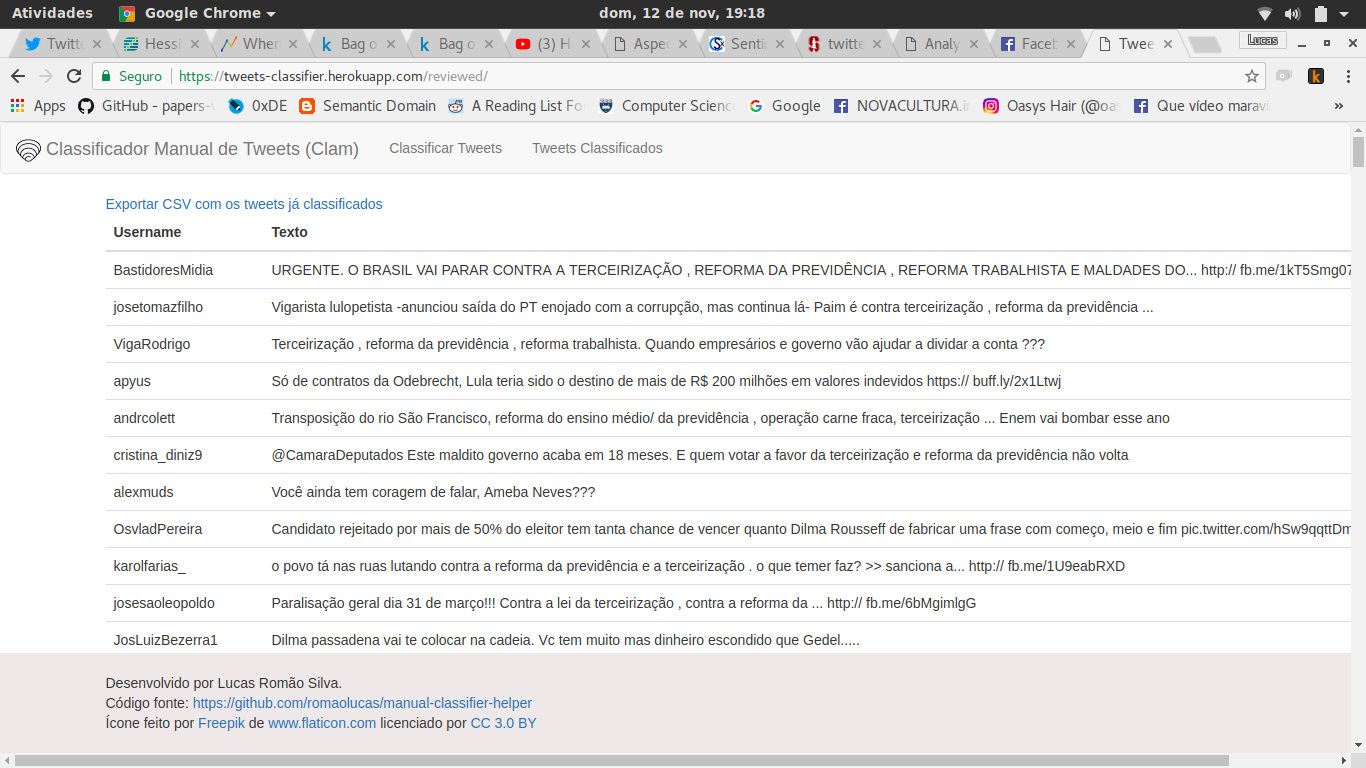
\includegraphics[scale=0.27]{clam_classificados}
	\end{figure}
\end{enumerate}

Para um usuário que deseja hospedar a plataforma e usá-la para si, existe também o admin onde
é possível importar \textit{tweets} para serem classificados.

Abaixo é descrito o fluxo para a importação de novos dados no admin.

\begin{enumerate}
	\item Realiza o login no sistema utilizando seu usuário e senha de administrador.
	\begin{figure}[H]
		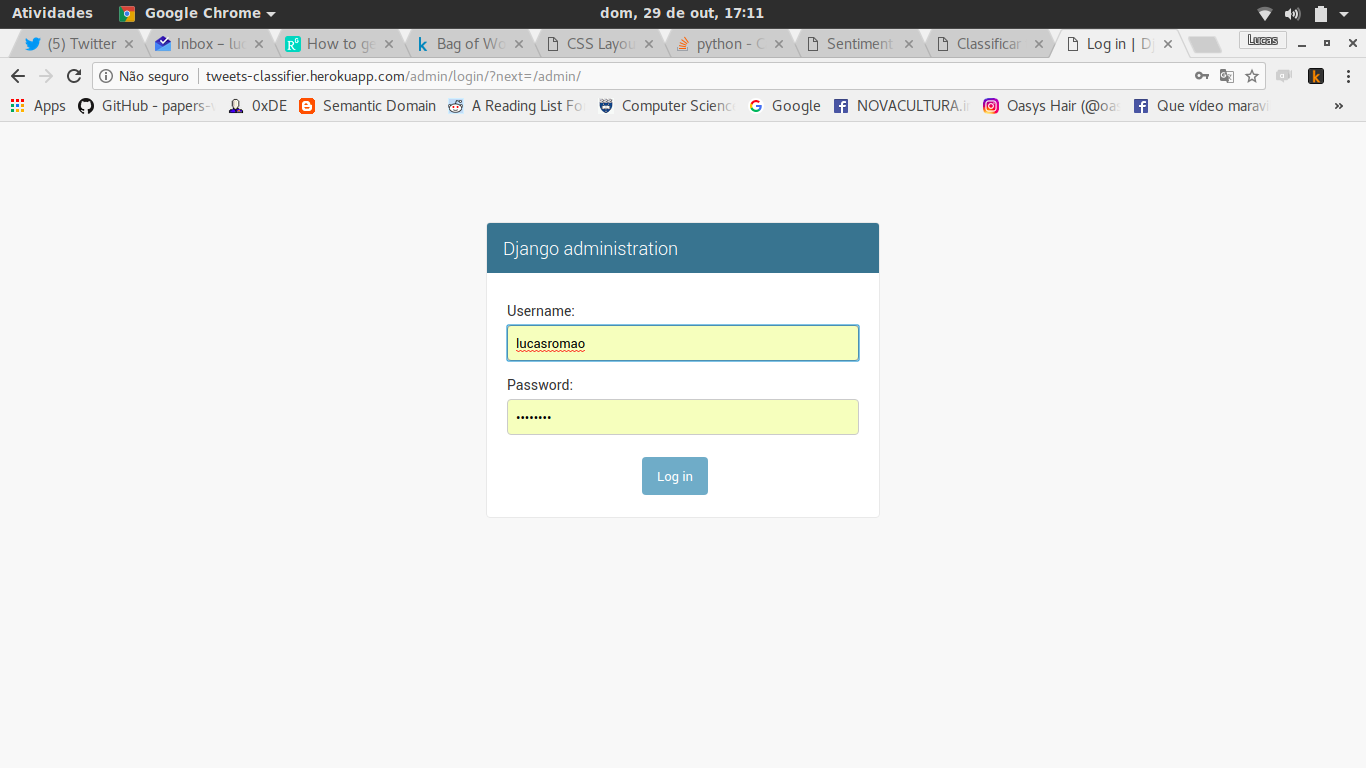
\includegraphics[scale=0.27]{clam_login}
	\end{figure}
	\item Seleciona a parte de Tweets na tela principal.
	\begin{figure}[H]
		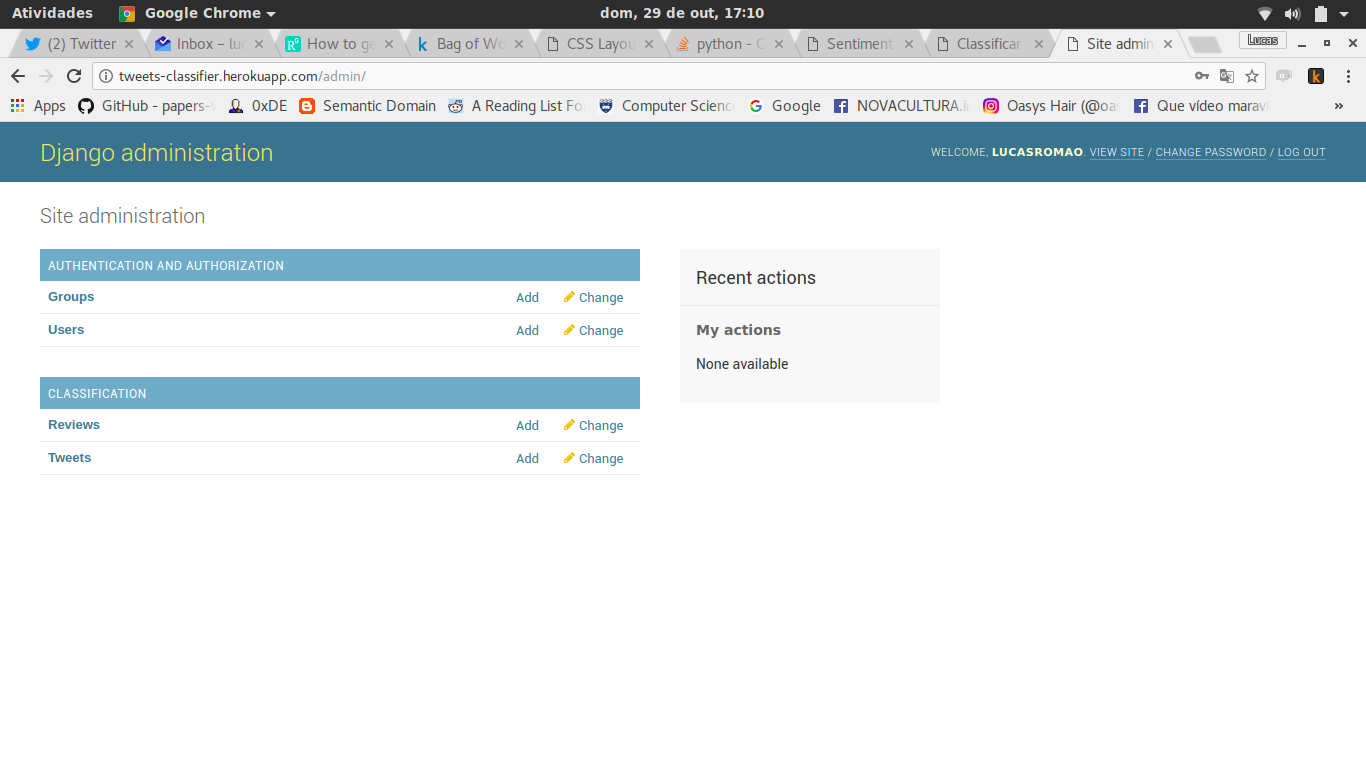
\includegraphics[scale=0.27]{clam_admin}
	\end{figure}
	\item Uma vez na parte de visualizar todos os \textit{tweets} já armazenados na base de dados,
	seleciona a opção de importar no canto superior direito.
	\begin{figure}[H]
		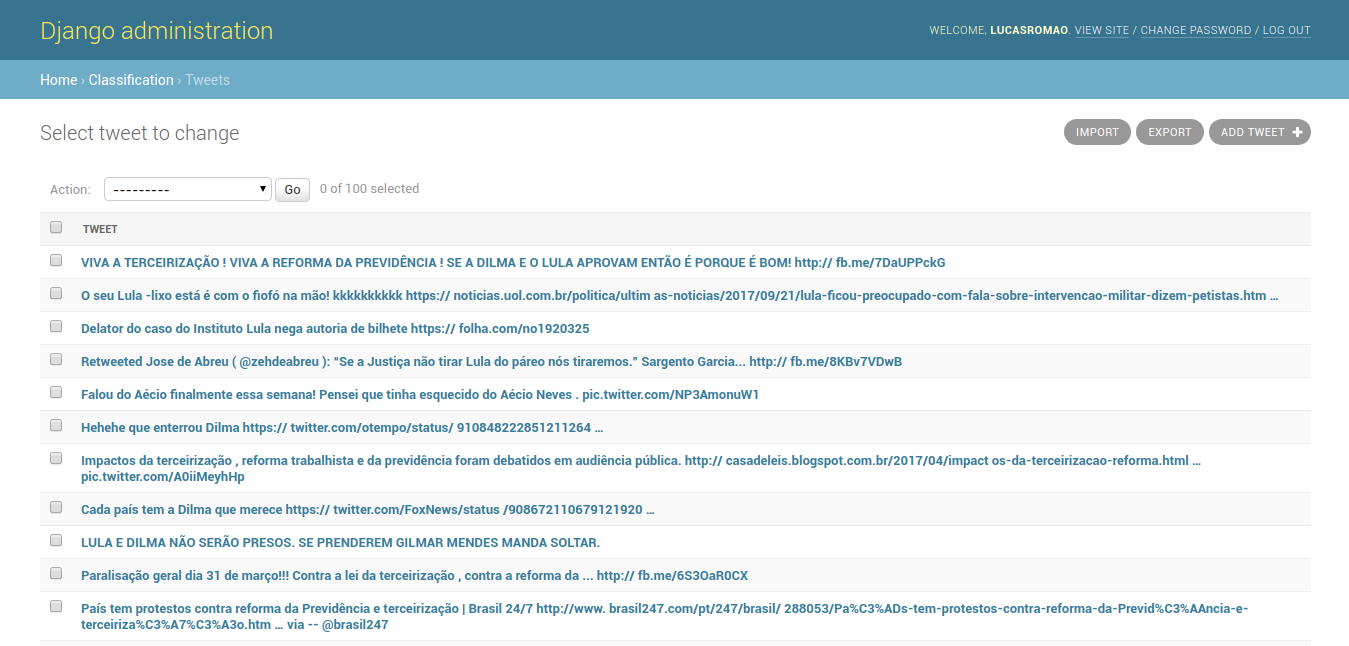
\includegraphics[scale=0.27]{clam_tweets}
	\end{figure}
	\item Na página que segue, basta informar um arquivo .csv, .xls (formato do excel) ou .json
	contendo nessa ordem: o id do \textit{tweet} (fornecido pelo Twitter), usuário que escreveu, 
	texto, espaço vazio para representar o id que será preenchido automaticamente na hora de 
	importar no banco de dados.
	\begin{figure}[H]
		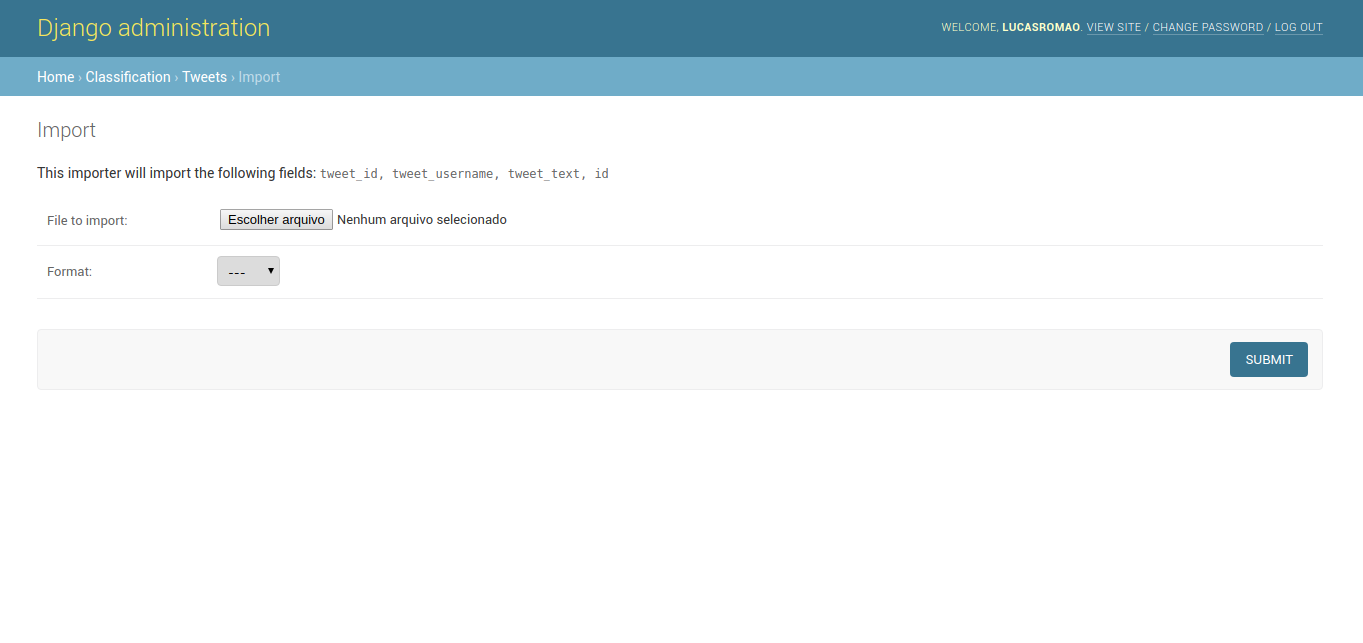
\includegraphics[scale=0.2]{clam_importador}
	\end{figure}
	\item Caso todos os dados sejam fornecidos corretamente, será passado a uma nova página para
	confirmar se deseja importar e, por fim, será redirecionado à pagina que contém todos os
	\textit{tweets}.
\end{enumerate}

